\chapter{Conclusion}

In conclusion, the goals of this project have been largely accomplished. The implementation of a Python routine for complete automation and integration of the system has significantly improved the precision of experiments and enabled real-time collection of extensive data without requiring the expertise and time of a specialized scientist. The success of this project underscores the potential of automation in enhancing scientific research and accelerating progress towards achieving research goals.
In addition to its potential in scientific research, the software developed in this project can also be leveraged by industrial approaches. Furthermore, the classification methods and system control implemented in this project have yielded promising results and can be further optimized in the future. Overall, this project serves as a valuable contribution towards the advancement of automated systems and the optimization of experimental processes, with broad implications for both research and industrial applications.

The works therefore presented here are a continuation and optimization of the routine to make it more precise and applicable to both industrial and research approaches.
The previous student work was more focused on detecting corona streamers or spark discharges, therefore her automation routine was a first version concept that proved to be valuable.
From the work I've done it highlights:

- Integrate liquid pump to the software and developed a routine with it.

- Modeled the software to fit a control model turning it easy to implement new control algorithms or experiment routines.

- Remodel the software to support threads in order to separate each subsystem and exchange data between them with use of queues data structures.

- Developed a classification for multi jet spraying mode.

- Developed a simple controller to proof the concept.

- Optimize the saving of data to a real time streaming together with more sensors' data.

- Restructured algorithm usability in order to make it more intuitive with the setup file.


\section{Proposal for continuing}

\subsection{Fuzzy Controller}

        The fuzzy approach of controller was explored and simulated but not used in the final version of the project.
        This because for this fuzzy approach we need to have the input variables for the fuzzy machine to be fuzzyfied.
        Which means that to use a fuzzy logic in our controller loop the classification must be fuzzyfied and our classification algorithm was not developed in order to give a classification and its current membership function.

        For that, I tried to fuzzyfy the controller input by the data acquired in the step routine. With the data I mapped the area of each spraying mode according to its potential and fuzzyfied this as shown in the Figure X.

        \begin{multicols}{2}

            \begin{figure}[H]
                \centering
                \resizebox{90mm}{!}{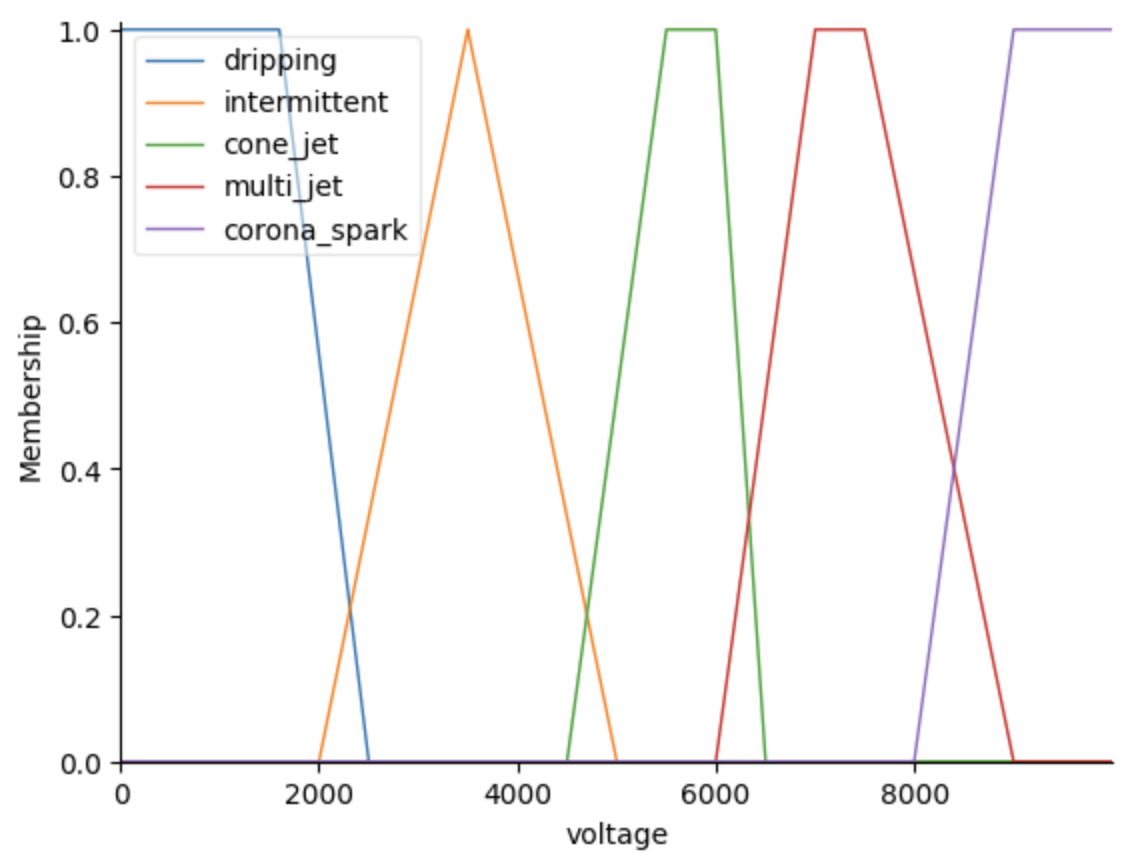
\includegraphics{Figuras/fuzzy/fuzzyfy_input.png}}
                \caption{Fuzzyfication}
                \label{fig:fuzzy_input}
            \end{figure}

            \begin{figure}[H]
                \centering
                \resizebox{90mm}{!}{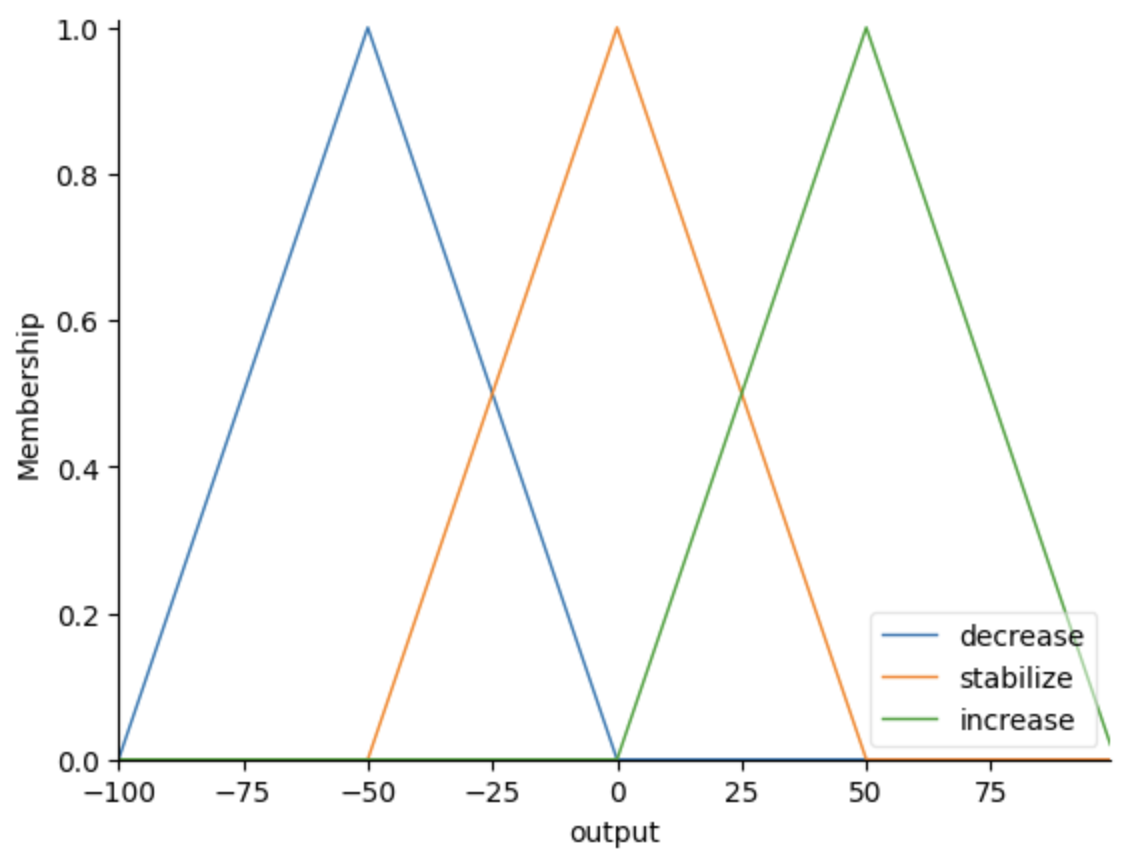
\includegraphics{Figuras/fuzzy/defuzzyfy.png}}
                \caption{Defuzzyfication}
                \label{fig:fuzzy_output}
            \end{figure}

        \end{multicols}

        \begin{figure}[H]
            \centering
            \resizebox{80mm}{!}{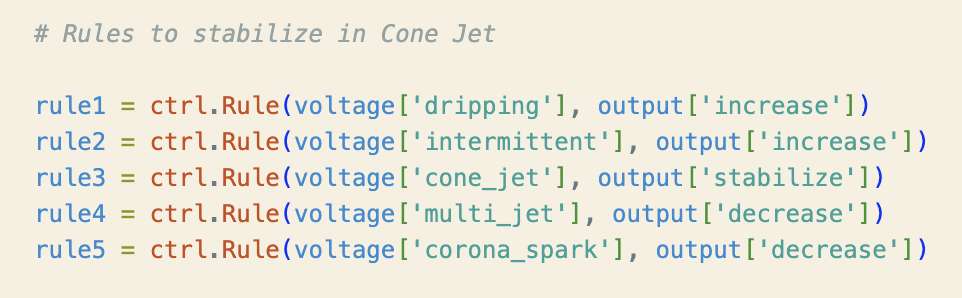
\includegraphics{Figuras/fuzzy/rules.png}}
            \caption{Fuzzy Rules}
            \label{fig:fuzzy_rules}
        \end{figure}

        \begin{multicols}{2}

            \begin{figure}[H]
                \centering
                \resizebox{90mm}{!}{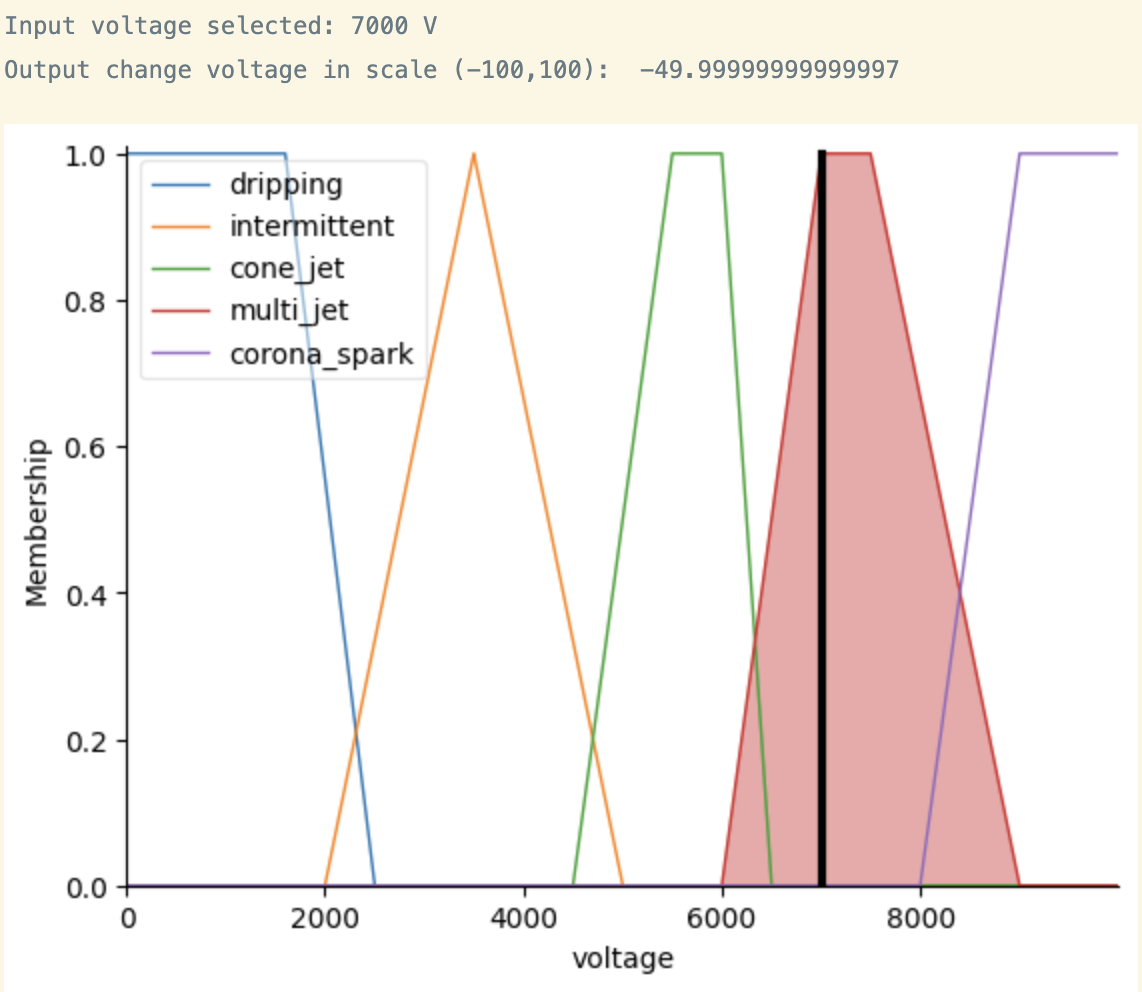
\includegraphics{Figuras/fuzzy/test1.png}}
                \caption{Test 1: fuzzy controller}
                \label{fig:fuzzy_test1}
            \end{figure}

            \begin{figure}[H]
                \centering
                \resizebox{90mm}{!}{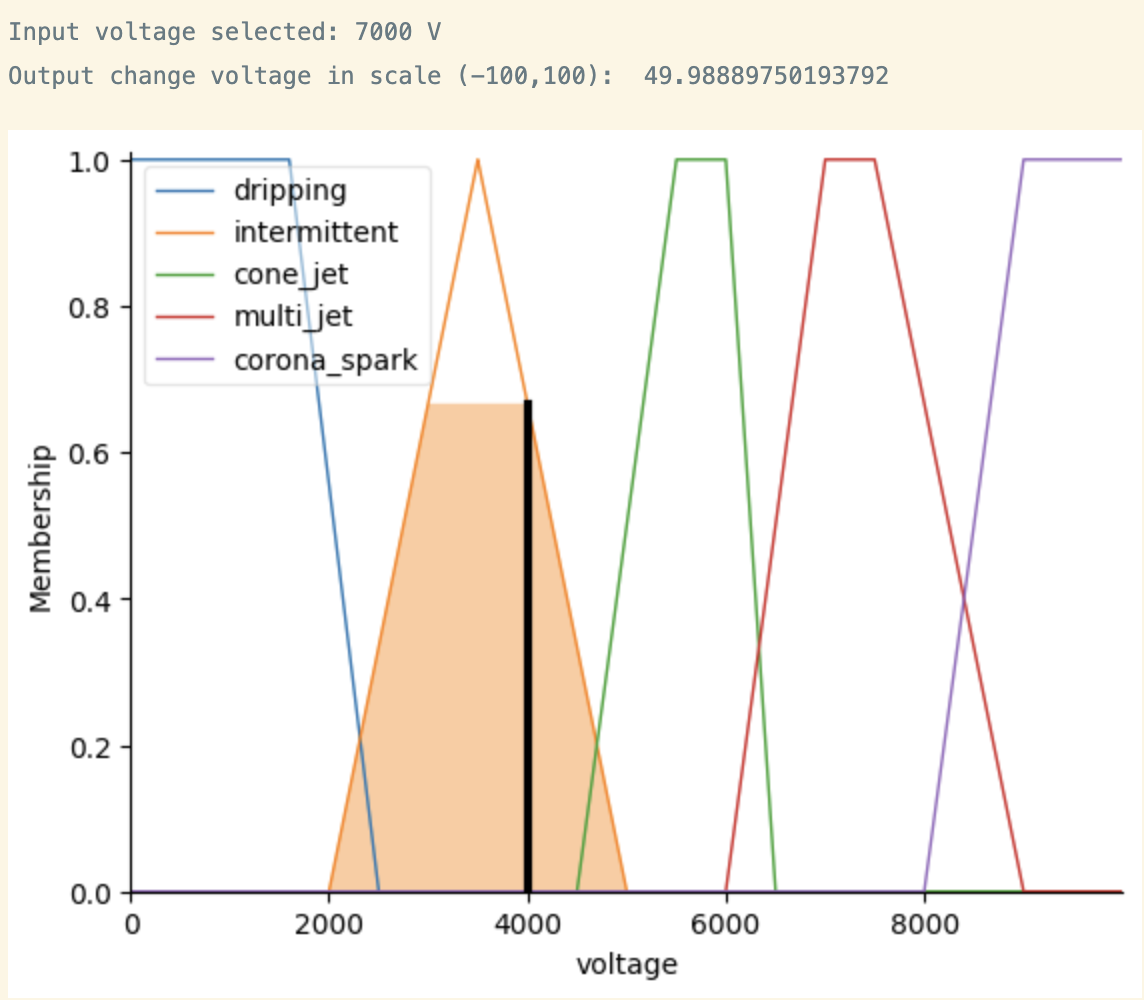
\includegraphics{Figuras/fuzzy/test2.png}}
                \caption{Test 2: fuzzy controller}
                \label{fig:fuzzy_test2}
            \end{figure}

        \end{multicols}
        

\clearpage
